\documentclass[11pt,a4paper]{article}
\usepackage[latin1]{inputenc}
\usepackage[spanish]{babel}
\usepackage{amsmath}
\usepackage{amsfonts}
\usepackage{amssymb}
\usepackage{graphicx}
%\usepackage{subfigure} % subfiguras
\usepackage[left=3.00cm, right=2.00cm, top=2.00cm, bottom=2.00cm]{geometry}
\author{Edwar Diaz Ruiz, eddiazr@correo.udistrital.edu.co, 20141020004 \\
liz}
\title{FORMATO IEEE INFORME}
\date{} % para la fecha
\usepackage{multicol}



\begin{document}
	\maketitle
	\begin{multicols}{2}
		\begin{abstract}
Este es un resumen de prueba para el formato ieee espero que todo quede bien...e en seguida colocare las palabras clave :D \\

	\smallskip
\textbf{palabras clave: } resumen, formato, ieee, sismtemas operativos
		\end{abstract}
%		\begin{center}
%			\textbf{RESUMEN}
%		\end{center}
%	Este es un resumen de prueba para el formato ieee espero que todo quede bien...e en seguida colocare las palabras clave :D\\
	
%	\smallskip
%	\textbf{palabras clave: } resumen, formato, ieee, sismtemas operativos
	%\section{INTRODUCCION}
	\begin{center}
		\section{INTRODUCCION}
		
	%	\textbf{INTRODUCCION}
	\end{center}
	En este epacio se colocara la introduccion a los informes futuros a realizar con la espera de que el formato quede bien hecho  para su futuro uso
	\smallskip
%	\begin{center}
%		\section{OBJETIVOS}
%		%\textbf{OBJETIVOS}
%	\end{center}
	\begin{center}
		\section{OBJETIVOS}
	%	\textbf{INTRODUCCION}
	\end{center}
	\begin{itemize}{}
		\item aqui se colocan objetivos
		\item aqui se colocan objetivos 2
	\end{itemize}
	
	\smallskip
	\begin{center}
		%\textbf{MARCO TE�RICO}
		\section{MARCO TE�RICO}
	\end{center}
	En esta seccion se agrega toda la teoria relevante para el informe no se debe agregar teoria por que si solo lo que este directamente relacionado con el informe tambien se pueden incluir imagenes formulas y demas, procurare colocar ejemplos.
	
	tambien se debe referencias todo lo que se agregue
	


\begin{minipage}{.8\linewidth}
	\centering
	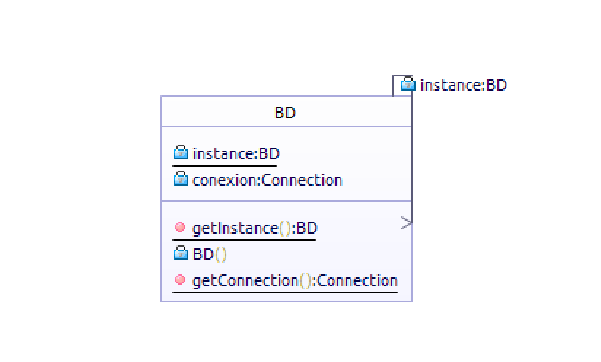
\includegraphics[width=6.0cm]{Singleton}
	\label{thelabel}
	\figurename{ prueba 1}
\end{minipage}

\medskip
	Tambien se pueden agregar pdf jpg y otros y no es necesario colocar la extencion que en este caso fue jpg, pero es mas aconsejable usar pdf yo lo recomiendo dejar la imagen o lo que sea en formato pdf, tambien dependiendo de la imagen deben de jugar con el tama�o aun no puedo cuadrar algo decente para que diga figura abajo :D\\
	enseguida hare una formula simple creo que se use en S.O pero no esta de mas
	
	$$
	\alpha + \beta = \chi \eqno{(1)}
	$$

\smallskip
	\begin{center}
	%\textbf{PROCESOS}
		\section{PROCESOS}
	\end{center}
	Aqui colocaremos los procesos que vamos a relizar en el informe 

\smallskip
	\begin{center}
		\section{DESARROLLO}
	\end{center}
	Aqui colocaremos el desarrollo y sus respectivos pantallazos

\smallskip

\begin{thebibliography}{99}
	\bibitem{c1} {\scriptsize G. O. Young, oSynthetic structure of industrial plastics (Book style with paper title and editor),� 	in Plastics, 2nd ed. vol. 3, J. Peters, Ed.  New York: McGraw-Hill, 1964, pp. 15D64.}
	
	\bibitem{c2} {\scriptsize PARA algo online...tema de lo que dice,disponible en: $www.googe.com.co$}
\end{thebibliography}
	\end{multicols}
\end{document}